\documentclass[11pt,a4paper]{article}
\author{TalentSprint}
\date{}
\usepackage{verbatim}
\usepackage{fancyhdr}           % For header and footer
\usepackage{multicol}
\usepackage{colortbl}           % For coloured tables
\usepackage{setspace}           % For line height
\usepackage{seqsplit}           % Splits long words.
\usepackage{amsmath} 
\usepackage{graphicx}
\usepackage{array}
\usepackage{enumitem}
\usepackage{xcolor}
\usepackage[tikz]{bclogo}
\usepackage{textcomp}
\usepackage{listings}
\lstset{language=python,numbers=left,numberstyle=\tiny,numbersep=10pt,showstringspaces=false}
\headheight=14pt
\lhead{\nouppercase{}}
\rhead{\nouppercase{\leftmark}}

\newcommand*\lstinputpath[1]{\lstset{inputpath=#1}}
\lstinputpath{../Code/}
\graphicspath{{../Images/} {../ScreenShots/}}

\setcounter{tocdepth}{1}
\setlength\parindent{0pt}
\parskip=4pt
\newcommand{\Code}[1]{\textbf{\texttt{#1}}}

% Lengths and widths
\addtolength{\textwidth}{5cm}
\addtolength{\hoffset}{-1cm}
\setlength{\headsep}{-12pt} % Reduce space between header and content
\setlength{\headheight}{85pt} % If less, LaTeX automatically increases it
\renewcommand{\footrulewidth}{2pt} % Remove footer line
\renewcommand{\headrulewidth}{1pt} % Remove header line
\renewcommand{\seqinsert}{\ifmmode\allowbreak\else\-\fi} % Hyphens in seqsplit
% This two commands together give roughly
% the right line height in the tables
\renewcommand{\arraystretch}{1.3}
\onehalfspacing

% Commands
\newcommand{\SetRowColor}[1]{\noalign{\gdef\RowColorName{#1}}\rowcolor{\RowColorName}} % Shortcut for row colour
\newcommand{\mymulticolumn}[3]{\multicolumn{#1}{>{\columncolor{white}}#2}{#3}} % For coloured multi-cols
\newcolumntype{x}[1]{>{\raggedright}p{#1}} % New column types for ragged-right paragraph columns
\newcommand{\tn}{\tabularnewline} % Required as custom column type in use

% Font and Colours
\definecolor{HeadBackground}{HTML}{333333}
\definecolor{FootBackground}{HTML}{666666}
\definecolor{TextColor}{HTML}{333333}
\definecolor{DarkBackground}{HTML}{6B8E23} %{FD1AA8}
\definecolor{LightBackground}{HTML}{E8FED8} %D3FDC8
\definecolor{tit}{HTML}{FF6600}
\renewcommand{\familydefault}{\sfdefault}
\color{TextColor}
 \headsep = 25pt
% Header and Footer
\pagestyle{fancy}
\usepackage[headheight=110pt]{geometry}
\fancyhf{}% Clear header/footer

\fancyhead[r]{
\includegraphics[width = 4cm, height = 2cm]{TS-Logo.png}\hspace{0cm}}

%=================================TITLE=====================================
\fancyhead[l]{\Large{\bf{\textcolor{tit}{\textrm{Introduction to C}}}}}
%===========================================================================

\renewcommand{\headrulewidth}{0.4pt}% Default \headrulewidth is 0.4pt
\renewcommand{\footrulewidth}{0.4pt}% Default \footrulewidth is 0pt

\rfoot{Page \thepage}
\lfoot{COPYRIGHT \textcopyright TALENTSPRINT, 2015. ALL RIGHTS RESERVED.}




\begin{document}


%\chapter{Conditional Statements}
Decision making structures require that the programmer specify one or more conditions to be evaluated by the program, along with statement(s) to be executed if the condition is determined to be \texttt{true}, and optionally, another set of statements to be executed if the condition is \texttt{false}.

\begin{figure}[ht]

\begin{center}
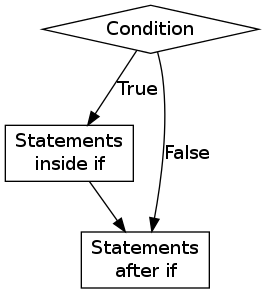
\includegraphics[scale=0.6]{if.png}
\caption{Control flow: if}
\label{Controlflow:if}
\end{center}
\end{figure}

\section {If Statement}
C uses the keyword \lstinline!if! to execute one or more statements when the condition is \texttt{true}. The \lstinline!if! statement controls conditional execution. The body of an \lstinline!if! statement is executed if the value of the expression is \texttt{true} (non-zero).

\subsubsection*{Syntax}
\begin{lstlisting}[numbers=none]
  if (boolean_expression) {
    statement(s);
  }
\end{lstlisting}
If the boolean expression evaluates to \texttt{true}, then the block of code inside the \lstinline!if! statement will be executed. If the boolean expression is \texttt{false}, then the code after the end of the \lstinline!if! statement will be executed.

\subsubsection*{Example} 
The next program checks whether the given number is positive, negative or zero. The output can be seen in Figure \ref{output-06-1}.

\lstinputlisting{Program-06-1.c}

\begin{figure}[ht]
\begin{center}
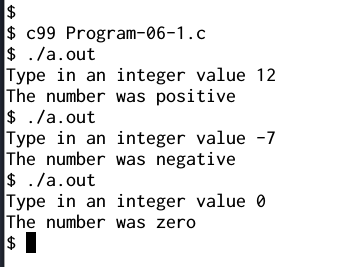
\includegraphics[scale=0.6]{Output-06-1.png}
\caption{Simple if}
\label{output-06-1}
\end{center}
\end{figure}

\subsection*{True/False in C}
Originally C did not have a boolean data type. C programming language treats any \texttt{non-zero} and \texttt{non-null} values as \texttt{true}.\texttt{zero} and \texttt{null}  are synonymous with \texttt{false}. Even \textbf{\texttt{c99}} adds a macro which essentially is a wrapper around the fact boolean is integral value.

So you may see code like \lstinline!while (1)! to set up an infinite loop. Modern programmers should use the symbolic constants \texttt{true} and \texttt{false} but should be prepared to read code where 1 (rarely some other non-zero value) stands for \texttt{true} and 0 for \texttt{false}.

\section*{If \ldots Else Statement}
C implements two-way selection with the \lstinline!if ... else! statement. It is a composite statement used to make a decision between two atlernatives. In other words, if the condition is true one set of statements is executed and if false, different piece of code is executed.

\subsubsection*{Syntax}
\begin{lstlisting}[numbers=none]
  if (boolean_expression) {
    A-statement(s); 
  } else {
    B-statement(s);
  }
\end{lstlisting}

In the above A-statement(s) are executed if the boolean\_expression is true; otherwise B-statement(s) are executed.

\begin{figure}[ht]
\begin{center}
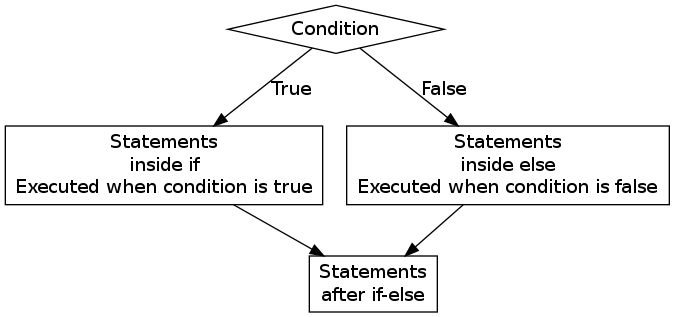
\includegraphics[scale=0.5]{ifelse.png}
\caption{Control flow: if else}
\label{ControlFlow:ifelse}
\end{center}
\end{figure}

To repeat, the \lstinline!if else! statement is a two way branch, it means do one thing or the other. When it is executed, the condition is evaluated and if it has the value `true' (i.e. not zero) then \lstinline!if! block statements will execute. If the condition is `false' (zero) then \lstinline!else! block statements will execute. 

\begin{lstlisting}[numbers=none]
  if (yy % 4 == 0) {
    nDays = 366;
  } else {
    nDays = 365;
  }
\end{lstlisting}

It is unnecessary to test whether yy is not divisible by 4 in the else block; since it is implied by the \emph{if-else} structure. That is, the block would be executed \emph{only} when the remainder is  NOT zero.

\subsection*{Example}

\lstinputlisting{Program-06-2.c}

\begin{figure}[ht]
\begin{center}
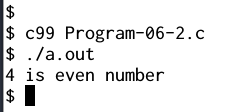
\includegraphics[scale = 0.6]{Output-06-2.png}
\caption{If else output}
\label{output-06-2}
\end{center}
\end{figure}

\section*{Complex Conditions}

So far we have written \lstinline!if! statements with simple conditions. They were simple boolean expressions. Similar to combining many operands with arithmetic operators for complex expressions, we can combine boolean expressions to create complex boolean expressions.

We saw an example where we tested \lstinline!yy % 4 == 0! to check if yy is a leap year. But as you probably know, the rule is more than that. A year is a leap year if it is divisible by 400 or is not divisible by 100 but divisible by 4.

To express the above in code we need to use logical operators. 

\section*{Logical Operators}
C has three logical operators for combining logical expressions and creating new logical expressions: \emph{not, and,} and \emph{or}. A common way to show logical relationships is using truth tables. Truth tables list the values that each operand can assume and the result of the expression.

\subsection*{Logical NOT}

The \emph{not} operator is \textbf{!}. It is an unary operator. It changes a \texttt{true} value to \texttt{false} and \texttt{false} value to \texttt{true}. That is, it toggles the value of the boolean expression it operates on.

\subsubsection*{Example}
\lstinputlisting{Program-06-3.c}

Of course the above example can be simplified. Line 6 can be rewritten as: \texttt{if (num < 0)} \ldots

\begin{figure}[ht]
\begin{center}
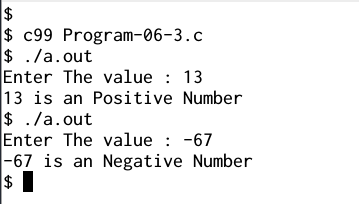
\includegraphics[scale=0.6]{Output-06-3.png}
\caption{Using NOT}
\label{output-06-3}
\end{center}
\end{figure}

\subsection*{Logical AND}
The \emph{and} operator is \&\&. It is a binary operator, used to combine multiple expresions, the result is \texttt{true} when \emph{all} expressions are \texttt{true}; \texttt{false} otherwise.

\subsubsection*{Example}
\lstinputlisting{Program-06-4.c}

\emph{The behaviour and output of this program is identical to the next code, where we rewrite the condition using $\mid\mid$}.

\subsection*{Logical OR} 
The \emph{or} operator is $\mid\mid$. It is a binary operator, used to combine multiple expressions. The result is \texttt{false} if all expressions are \texttt{false}, it is \texttt{true} in all other cases. Stated another way, it returns \texttt{true} if \emph{any one} of the component expressions is \texttt{true}.

\subsubsection*{Example}
\lstinputlisting{Program-06-5.c}

\begin{figure}[ht]
\begin{center}
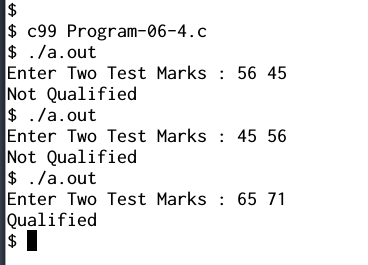
\includegraphics[scale=0.6]{Output-06-4.png}
\caption{Using Logical Operators}
\label{output-06-4}\end{center}
\end{figure}

\subsection*{Short-circuit Evaluation}
Computer languages use short-circut method to evaluate the binary logical relationships, it does not need to complete the evaluation. In other words, it operates in a short-circuit fashion and stops the evaluation as soon asit knows the final result for sure.

So if the first operand of a logical \emph{and} expression is \texttt{false}, the second half of the expression is not evaluated because it is apparent that the result must be \texttt{false}. Again, with the \emph{or} expression, if the first operand is \texttt{true}, then there is no need to evaluate the second half of the expression, so the resulting value is set to \texttt{true} immediately.

Recall the example of the leap year condition: a year is a leap year if it is divisible by 400 or it is not divisible by 100 but divisible by 4.

\texttt{isleap = (yy \% 400 == 0) || ((yy \% 100 != 0) \&\& (yy \% 4 == 0));}

\begin{description}
\item[yy is 2000] The first condition is \texttt{true}. So we need not evaluate what follows the $\mid\mid$, as (\texttt{true} $\mid\mid$ any) is \texttt{true}. That is 2000 is a leap year.

\item[yy is 1900] The first condition is \texttt{false}. So what follows the OR needs to be evaluated. The first part of that is \texttt{false}. So the part following AND is not evaluated as (\texttt{false} \&\& any) is \texttt{false}. The whole expression simplifies to (\texttt{false} $\mid\mid$ \texttt{false}) $\Rightarrow$ \texttt{false}. $\Rightarrow$ 1900 is NOT a leap year.

\item[yy is 2012] The first condition is \texttt{false}, but as it is followed by an OR the rest needs to be evaluated. That is also a complex condition. The first part is \texttt{true}. Still the part following the AND needs to be evaluated; that part is \texttt{true}. So the whole expressions simplifies to 

\texttt{false} $\mid\mid$ (\texttt{true} \&\& \texttt{true}) 

which is \texttt{true}. That is 2012 is a leap year.

\item[yy is 2014] The first condition is \texttt{false}, but as it is followed by an OR the rest needs to be evaluated. That is also a complex condition. The first part is \texttt{true}. Still the part following the AND needs to be evaluated; that part is \texttt{false}. So the whole expression simplifies to

\texttt{false} $\mid\mid$ (\texttt{true} \&\& \texttt{false}) 

which is \texttt{false}. That is 2014 is NOT a leap year.
\end{description}

\section*{Nested If Statement}

An \lstinline!if! statement within an another \lstinline!if! statement is termed as \emph{nested-if} statement. When the outer \lstinline!if! statement is satisfied then it will check for the inner \lstinline!if! statement and execute the block of code.

\subsection*{Syntax}
\begin{lstlisting}[numbers=none]
  if (A_boolean_expression) {   // Outer if 
    if (B_boolean_expression) { // Inner if 
      Alpha_statement;
    } else {
      Beta_statement;
    }
  } else {
    Gamma_statement;
  }
\end{lstlisting}

There is nothing special about a nested-if. An \lstinline!if! statement has a set of statements to be executed when the condition is true and optionally another set of statements to be executed when the condition is false. One or more of these statements in question can be an \lstinline!if! statement itself.

In above, the condition A\_boolean\_expression is checked first. If it is true, then the program control goes inside the braces and executes the next statement: which checks the next condition (inner if) namely B\_boolean\_expression. If it is also true then it executes the block of statements associated with it, namely Alpha\_statement; if not the Beta\_statement is executed; if the outer if is itself false, execution continues directly with Gamma\_statement.

We can build a Truth table to explain the flow:

\begin{tabular}{|c|c|c|}\hline
A\_boolean\_expression & B\_boolean\_expression & Action\\\hline
True                 & True                 & Alpha\_statement\\\hline
True                 & False                & Beta\_statement\\\hline
False                & Don't care           & Gamma\_statement\\\hline
\end{tabular}

\subsection*{Example}
Let us revisit the complex condition we wrote for the leap year. Let us rewrite it as a nested-conditional statement.

\texttt{isleap = (yy \% 400 == 0) || ((yy \% 100 != 0) \&\& (yy \% 4 == 0));}

\begin{lstlisting}
     if (yy % 400 == 0)
         isleap = true;
     else 
         if (yy % 100 == 0)
             isleap = false;
         else
             if (yy % 4 == 0)
                 isleap = true;
             else
                 isleap = false;
\end{lstlisting}

Trace the above for the four values, 2000, 1900, 2012, 2014 and convince yourself they are equivalent. Note that we can simplify the above code somewhat. 
\begin{lstlisting}
     if (yy % 400 == 0)
         isleap = true;
     else 
         if (yy % 100 == 0)
             isleap = false;
         else
             isleap =  (yy % 4 == 0);
\end{lstlisting}
Such use of boolean expressions is a good idea.

\subsubsection*{Another example}
\lstinputlisting{Program-06-6.c}

\section*{If \ldots Else Ladder}
It is a conditional statement which is used to check a series of conditions. Each condition is associated with a set of statements. The conditions are checked one after another. The code associated with the first true condition is executed. And then control goes out of the ladder.

\subsection*{Syntax} 
\begin{lstlisting}[numbers=none]
    if (boolean_expression1) {
        aStatement;
    } else if (boolean_expression2 ) {
        bStatement;
    } else if (boolean_expression3) {
        cStatement;   
    } else {
        catchall_statement;
    }
\end{lstlisting}

\begin{figure}[ht]

\begin{center}
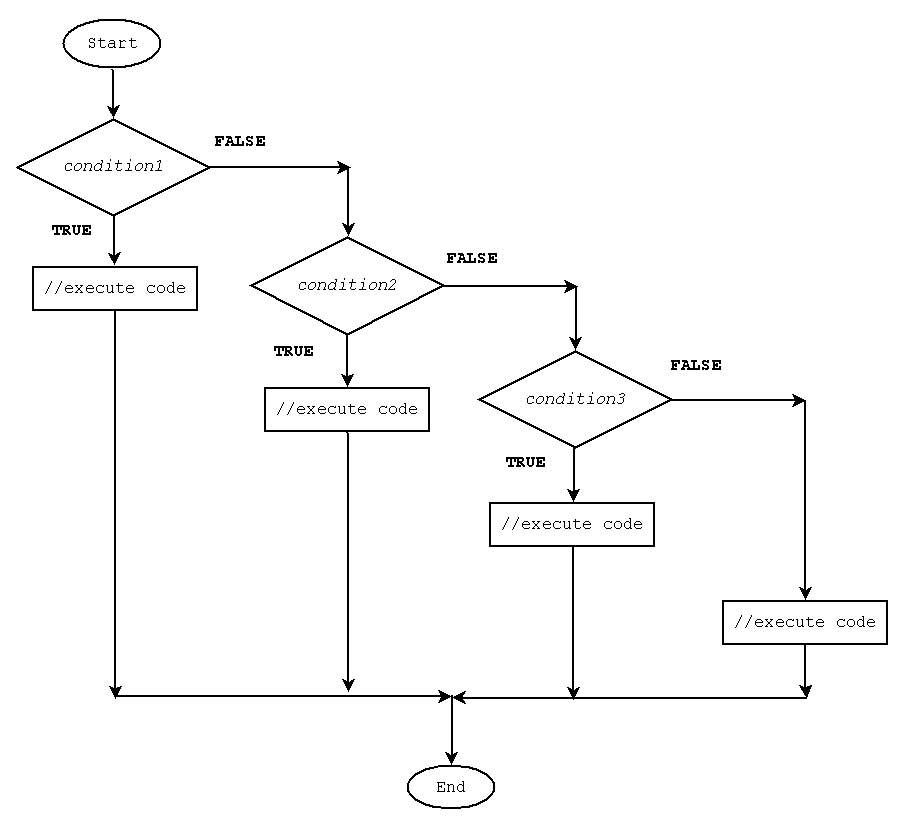
\includegraphics[scale=0.4]{flowchart_if-else-if-statement.png}
\caption{Flowchart if else ladder}
\label{Flowchart:ifelseladder}
\end{center}
\end{figure}

\subsection*{Example}
 
\lstinputlisting{Program-06-7.c}

\section*{Switch case}  
The switch statement is similar to the \lstinline!if! \ldots ~\lstinline!else! ladder statement. The switch makes one selection when there are several choices to be made. 

But the major difference between \lstinline!switch! \ldots ~\lstinline!case!, and a ladder is that the conditional expression must evaluate to an integer.

The general form of \lstinline!switch! statement is shown below:

\subsection*{Syntax}

\begin{lstlisting}[numbers=none]
  switch (expression) {
    case constant1:  
      statement 1;
      break;

    case constant2: 
      statement 2;
      break;

    case constantn: 
      statementn;
      break;

    default: 
      statement;
  }
\end{lstlisting}

The key word \lstinline!case! is followed by an integer or a character constant. Each constant in each case must be different from all others, that is, each case constant must be distinct.

The \lstinline!break! statement is used inside each case of the \lstinline!switch!, causes an immediate exit from the \lstinline!switch! statement; and execution continues from the statement after the \lstinline!switch! statement.

When we execute the \lstinline!switch! statement, first the expression is evaluated. The value of expression is then compared one-by-one, with constant1, constant2 \ldots constantn. When a match is found, the program executes the statements corresponding to that \lstinline!case!. 

The execution continues from that point till either a \lstinline!break! statement is found or the \lstinline!switch! statement is completed. The \lstinline!break! causes an immediate exit from the switch construct.

\begin{figure}[h]
\begin{center}
\includegraphics[scale=0.7]{{cswitchstatement.png}}
\caption{Flowchart: Switch Case}
\label{Flowchart:SwitchCase}
\end{center}
\end{figure}

\subsection*{Example}
 
\lstinputlisting{Program-06-8.c}

If the option selected is 1, then the output of this program is \ldots

	you selected first choice

	you selected second choice

	you selected third choice

\begin{bclogo}[couleur=blue!5, arrondi=0.3, logo=\bcbombe]{Missing Break in Switch}
Because there is no \lstinline!break! statement in the corresponding cases, the execution of the switch statement continues to all subsequent cases (including default if exist).
\end{bclogo}

\subsection*{Example}
 
The following program reads two numbers and performs selected arithmetic operation.
\lstinputlisting{Program-06-9.c}

\begin{figure}[ht]
\begin{center}
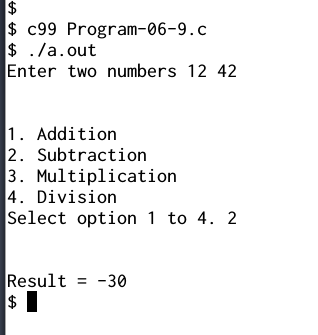
\includegraphics[scale=0.5]{Output-06-9.png}
\caption{switch case calculator}
\label{Switch:calculator}
\end{center}
\end{figure}
\end{document}